\documentclass{report}

\usepackage[utf8]{inputenc}
\usepackage[T1]{fontenc}
\usepackage[francais]{babel}
\usepackage{listings}
\usepackage[a4paper]{geometry}
\usepackage{graphicx}
\usepackage{titlesec}
\usepackage{color}

\definecolor{xcodekw}{rgb}{0.75, 0.22, 0.60}
\definecolor{xcodestr}{rgb}{0.89, 0.27, 0.30}
\definecolor{xcodecmt}{rgb}{0.31, 0.73, 0.35}

\titleformat{\chapter}[display]
  {\centering\normalfont\huge\bfseries}
  {\chaptertitlename\ \thechapter}
  {20pt}
  {\Huge}

\geometry{hscale=0.75,vscale=0.85,centering}

\DeclareUnicodeCharacter{00A0}{ }

\lstset{
  frame=tb,
  language=C,
  aboveskip=3mm,
  belowskip=3mm,
  showstringspaces=false,
  columns=flexible,
  basicstyle={\small\ttfamily},
  numbers=none,
  breaklines=true,
  breakatwhitespace=true,
  tabsize=3,
  keywordstyle=\color{xcodekw},
  stringstyle=\color{xcodestr},
  commentstyle=\color{xcodecmt}
}

\renewcommand{\thesection}{\arabic{section}}
\title{Projet OS}
\author{Youri \bsc{Mouton}, Rémy \bsc{Voet} et Samuel \bsc{Monroe}}
\date{Janvier 2015}

\begin{document}

\maketitle

\chapter{Introduction}

	\section{Introduction}

		Le projet qui fait l'objet de ce rapport est un travail de programmation
		en C système sous UNIX, dans le but d'exploiter de manière pratique les connaissances théoriques acquises au cours de Mme. Masson.
		\newline

		Ce travail consiste en l'écriture de trois programmes distincts autour d'une thématique aéronautique, échangeant des informations entre eux via divers moyens, ceci tout en gérant les éventuels conflits et erreurs liés à ces échanges.\newline
		Ces trois programmes sont :\newline
		\begin{description}
			\item[Tour de controle : ]
			Fait office de \textbf{serveur}, joue le rôle majeur en s'occupant de recevoir les demandes des pilotes, en allant chercher les informations météo fournies par le centre météo, et en renvoyant celles-ci en tant que réponses aux demandes des pilotes.

			\item[Pilote : ]
			Fait office de \textbf{client}, envoie une demande d'information ATIS à la tour de contrôle, récupère cette information et replace une demande si cette information n'est pas intègre.

			\item[Le centre météo : ]
			Programme \textbf{tiers} dans l'application, celui-ci se charge de générer automatiquement des informations ATIS différentes tout au long de son fonctionnement.
		\end{description}

	\section{Rappel de l'énoncé}

		Des pilotes qui souhaitent décoller d’un aéroport non contrôlé ont besoin, pour ce faire, de connaître les informations ATIS. Celles-ci sont accessibles via un serveur.
		Chaque pilote va envoyer au serveur une demande ATIS. Le serveur va lors répondre à cette demande en allant chercher les informations nécessaires dans un fichier ATIS.
		Le pilote va recevoir ces informations et il doit alors obligatoirement répondre au serveur en lui envoyant soit :\newline
		\begin{itemize}
			\item Un NAK OK qui signifie \og informations bien reçues \fg et provoque la fin de la communication
			\item Un ACK KO qui signifie \og informations mal comprises \fg et nécessite de renvoyer les informations.
		\end{itemize}

		Le serveur doit pouvoir gérer un nombre indéfini de pilotes (restons réalistes).
		Le fichier ATIS contenant les informations nécessaires aux pilotes doit être régulièrement mis à jour par le gestionnaire météo.

\chapter{Analyse}
 \section{Plan de l'application}
	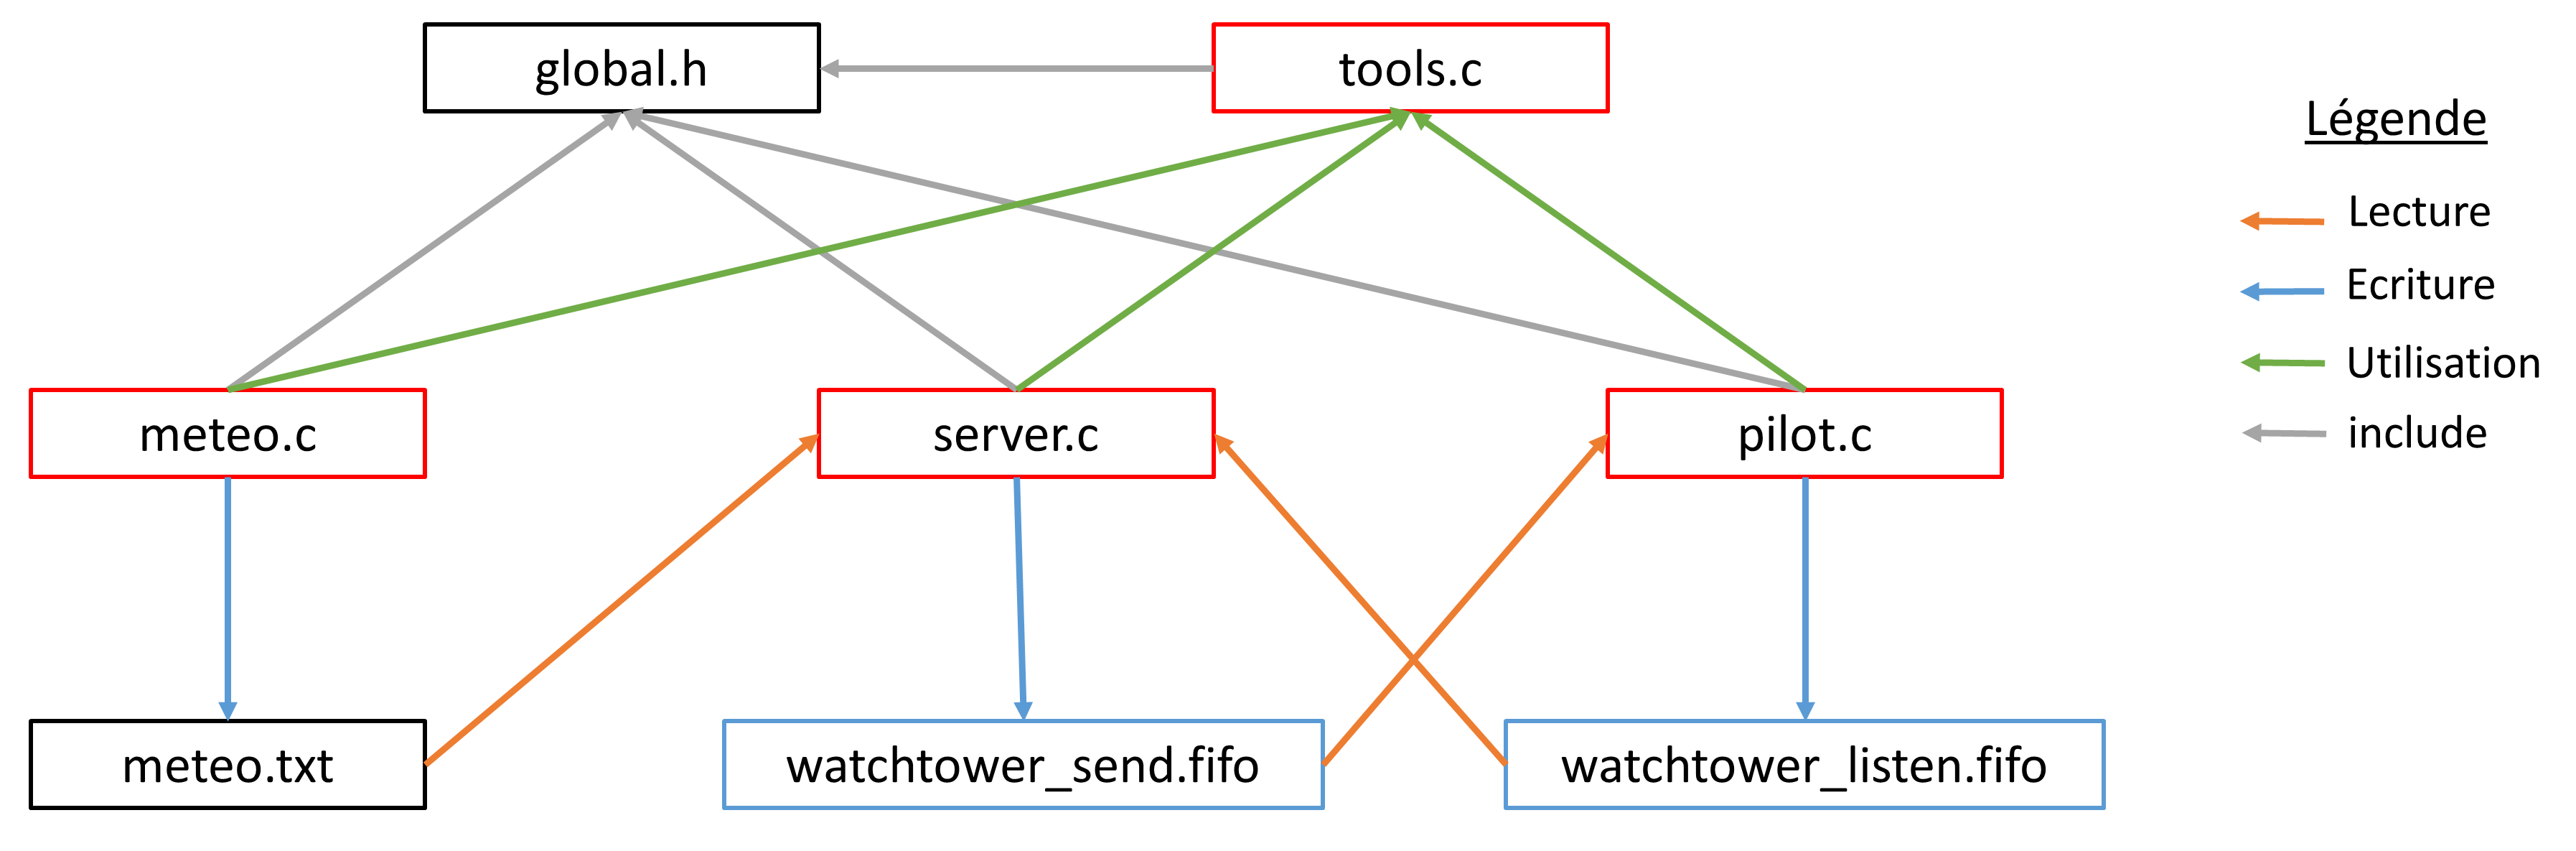
\includegraphics[width=450px]{schemasProjet.png}
	
\chapter{Détails des élements techniques spécifiques}
\chapter{Conclusion}
\appendix

\chapter{global.h}
	\lstinputlisting[language=C]{../global.h}
\chapter{meteo.c}
	\lstinputlisting[language=C]{../meteo.c}
\chapter{pilot.c}
	\lstinputlisting[language=C]{../pilot.c}
\chapter{server.c}
	\lstinputlisting[language=C]{../server.c}
\chapter{tools.c}
  \lstinputlisting[language=C]{../tools.c}
\tableofcontents

\end{document}